\section{二叉树}

\begin{frame}\ft{二叉树}
\begin{dingyi}
二叉树(Binary tree)是$n(n\ge0)$个结点的有限集合。
当$n=0$时称为空树,否则
\begin{itemize}
\item[(1)]有且只有一个特殊的称为树的根(Root)结点;
\item[(2)]当$n>1$时,其余结点被分成两个互不相交的子集$T_1,T_2$,
分别称之为左、右子树,并且左、右子树又都是二叉树。
\end{itemize}
由此可知,二叉树的定义是递归的。
\end{dingyi}
\end{frame}

%
%
\begin{frame}\ft{二叉树}
二叉树在树结构中起着非常重要的作用。因为二叉树结构简单,存储效率高,树的操作算法相对简单,且任何树都很容易转化成二叉树结构。上节中引入的有关树的术语也都适用于二叉树。
\end{frame}
%
\begin{frame}\ft{二叉树}
\textcolor{acolor5}{二叉树的特点:}
  \begin{itemize}
  \item 每个结点最多有两棵子树,所以二叉树不存在度大于$2$的结点。
  %\item[] {\bf 注:} 不是只有两棵子树,而是最多有。没有子树或有一棵子树都是可以的。\\[0.1in]
  \item 左子树和右子树是有顺序的,次序不能任意颠倒。\\[0.1in]
  \item 对于树中的某结点,即使只有一棵子树,也要区分它是左子树还是右子树。
  \end{itemize}
\end{frame}

\begin{frame}\ft{二叉树}%\fst{二叉树的基本形态}

\begin{figure}
\centering
\begin{tikzpicture}[scale=0.8]

  \node[] at (0,0) {$\Huge \varnothing$};
  \node[above] at (0,0.5){空二叉树};

  \node[circle,draw,text width=0.3cm] at (2.5,0) {};
  \node[above,text width=1.5cm] at (2.5,0.5){单结点二叉树};


  \node[circle,draw,text width=0.3cm] at (6,0) {}  
  child {node[circle,draw,text width=0.3cm]{} }
  child[fill=none] {edge from parent[draw=none]};  
  \node[above,text width=1.5cm] at (6,0.5){右子树为空};

  \node[circle,draw,text width=0.3cm] at (9,0) {}
  child[fill=none] {edge from parent[draw=none]}
  child {node[circle,draw,text width=0.3cm]{} };
  \node[above,text width=1.5cm] at (9,0.5){左子树为空};

  \node[circle,draw,text width=0.3cm] at (12,0) {}
  child {node[circle,draw,text width=0.3cm]{} }
  child {node[circle,draw,text width=0.3cm]{} };  
  \node[above,text width=1.5cm] at (12,0.5){左、右子树都不空};

\end{tikzpicture}

\caption{二叉树的5种基本形态}
\end{figure}

\end{frame}
%
\begin{frame}\ft{特殊二叉树}
 1、斜树
 \begin{itemize}
  \item 所有结点都只有左子树的二叉树叫左斜树;所有结点都只有右子树的二叉树叫右斜树。%\pause 
  \item \textcolor{acolor5}{特点:} 每一层都只有一个结点,结点的个数与二叉树的深度相同。%\pause 
  \item 这与线性表结构相同。其实线性表结构可以理解为树的一种极其特殊的表现形式。
  \end{itemize}
\end{frame}
%
%
\begin{frame}\ft{特殊二叉树}
2、满二叉树

在一棵二叉树中,如果所有分支结点都存在左子树和右子树,并且所有叶子都在同一层,这样的二叉树称为满二叉树。


% \begin{block}{满二叉树}
% 一棵深度为$k$且有$2k-1$个结点的二叉树称为满二叉树(Full Binary Tree)。
% \end{block}

\begin{figure}
\centering
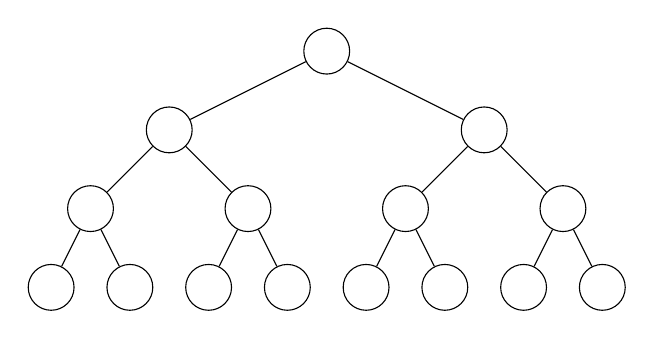
\begin{tikzpicture}[level distance=10mm]
  \tikzstyle{every node}=[circle,text width=0.3cm]
  \tikzstyle{level 1}=[sibling distance=4cm]
  \tikzstyle{level 2}=[sibling distance=2cm]
  \tikzstyle{level 3}=[sibling distance=1cm]
  \node[circle,draw] {} 
  child{node[circle,draw]{} 
    child{node[circle,draw]{} 
      child{node[circle,draw]{}}
      child{node[circle,draw]{}}
    }
    child{node[circle,draw]{} 
      child{node[circle,draw]{}}
      child{node[circle,draw]{}}
    }
  }
  child{node[circle,draw]{} 
    child{node[circle,draw]{} 
      child{node[circle,draw]{}}
      child{node[circle,draw]{}}
    }
    child{node[circle,draw]{} 
      child{node[circle,draw]{}}
      child{node[circle,draw]{}}
    }
  };

\end{tikzpicture}

%\caption{满二叉树}
\end{figure}•
\end{frame}
%
%
\begin{frame}\ft{特殊二叉树}
\textcolor{acolor5}{满二叉树的特点:}
\begin{itemize}
\item 
叶子只能出现在最下一层。
\item 
非叶子结点的度一定是$2$。
\item 
若深度为$k$,则结点数为$2^k-1$。在同样深度的二叉树中,满二叉树的结点个数最多,叶子数最多。
\item   
可对满二叉树的结点进行连续编号,若规定从根结点开始,按“自上而下、自左至右”的原则进行。
\end{itemize}

\end{frame}
%
%
\begin{frame}\ft{\subsubsecname}
  3、完全二叉树 (Complete Binary Tree)
  
%   对一棵具有$n$个结点的二叉树按层序编号,如果编号为$i(1\le i \le n)$的结点与同样深度的满二叉树中编号为$i$的结点在二叉树中位置完全相同,则这棵二叉树称为完全二叉树。


对一棵深度为$k$、结点数为$n$的二叉树按层序编号,若编号$i(1\le i \le n)$的结点与同样深度的满二叉树中编号为$i$的结点在二叉树中位置完全相同,则该二叉树称为完全二叉树。
%\vspace{0.1in}
%
% 或深度为k的满二叉树中编号从1到n的前n个结点构成了一棵深度为k的完全二叉树,其中$2^{k-1}\le n \le 2^k-1$。
%\end{frame}
%
%
% \begin{frame}\ft{\subsubsecname}
\begin{figure}
\centering
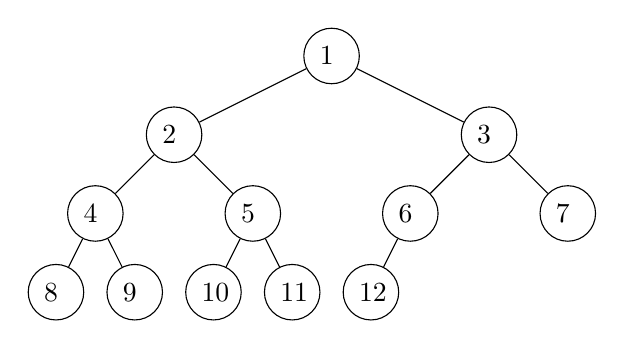
\begin{tikzpicture}[level distance=10mm]
  \tikzstyle{every node}=[circle,draw,text width=0.3cm]
  \tikzstyle{level 1}=[sibling distance=4cm]
  \tikzstyle{level 2}=[sibling distance=2cm]
  \tikzstyle{level 3}=[sibling distance=1cm]
  \node {1}
  child {node {2}
    child {node {4}
      child {node {8}}
      child {node {9}}
    }
    child {node {5}
      child {node {10}}
      child {node {11}}
    }
  }
  child {node {3}
    child {node {6}
      child {node {12}}
      child[fill=none] {edge from parent[draw=none]}
    }
    child {node {7}}
  };
\end{tikzpicture}

%\caption{完全二叉树}
\end{figure}
\end{frame}
%
\begin{frame}\ft{\subsubsecname}
\begin{figure}
\centering
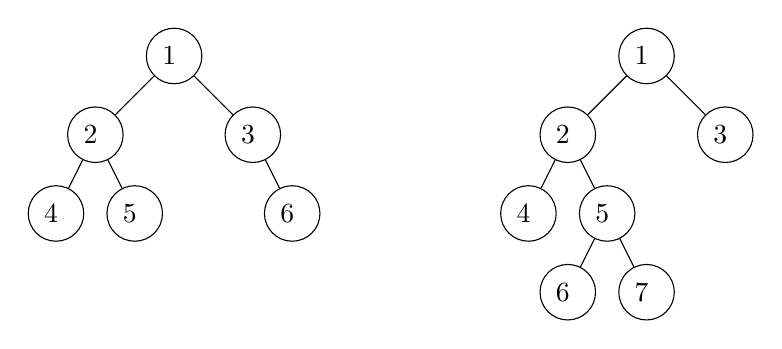
\begin{tikzpicture}[level distance=10mm]
  \tikzstyle{every node}=[circle,draw,text width=0.3cm]
  \tikzstyle{level 1}=[sibling distance=2cm]
  \tikzstyle{level 2}=[sibling distance=1cm]
  \tikzstyle{level 3}=[sibling distance=1cm]
  \node at (2,0) {1}
     child {node {2}
       child {node {4}}
       child {node {5}}
     }
     child {node {3}
       child[fill=none] {edge from parent[draw=none]}
       child {node {6}}
     };

   \node at (8,0) {1}
     child {node {2}
       child {node {4}}
       child {node {5}
         child {node {6}}
         child {node {7}}
      }
     }
     child {node {3}};
\end{tikzpicture}

\caption{非完全二叉树}
\end{figure}
\end{frame}
%
\begin{frame}\ft{\subsubsecname}
完全二叉树是满二叉树的一部分,而满二叉树是完全二叉树的特例。

\textcolor{acolor5}{满二叉树的特点}
% 若完全二叉树的深度为$k$,则所有的叶子结点都出现在第$k$层或$k-1$层。对于任一结点,如果其右子树的最大层次为$l$,则其左子树的最大层次为$l$或$l+1$。
  \begin{itemize}
  \item 叶子结点只能出现在最下两层。
  \item 最下层的叶子一定集中在左部连续位置。
  \item 倒数第二层,若有叶子结点,一定都在右部连续位置。
  \item 如果结点度为1,则该结点只有左孩子,即不存在只有右子树的情况。
  \item 同样结点数的二叉树,完全二叉树的深度最小。
  \end{itemize}


\end{frame}
%
%
\begin{frame}\ft{二叉树的性质}
\begin{xingzhi}[1]
在非空二叉树中,第$i$层上至多有$2^{i-1}$个结点($i\ge 1$)。
\end{xingzhi}

\begin{itemize}
\item 第一层是根节点,只有一个,$2^{1-1}=2^0=1$。
\item 第二层有两个,$2^{2-1}=2^1=2$。
\item 第三层有两个,$2^{3-1}=2^2=4$。
\item 第四层有两个,$2^{4-1}=2^3=8$。
\end{itemize}
利用数学归纳法,容易得出在二叉树的第$i$层上至多有$2^{i-1}$个结点($i\ge 1$)。
\end{frame}
%
%
\begin{frame}\ft{二叉树的性质}
\begin{xingzhi}[2]
深度为$k$的二叉树至多有$2^k-1$个结点($k\ge1$). 
\end{xingzhi}

\begin{itemize}
\item 如果有一层,至多$1=2^1-1$个结点。
\item 如果有二层,至多$1+2=3=2^2-1$个结点。
\item 如果有三层,至多$1+2+4=2^3-1$个结点。
\item 如果有四层,至多$1+2+4+8=2^4-1$个结点。
\end{itemize}
利用数学归纳法,容易得出,如果有$k$层,此二叉树至多有$2^{k}-1$个结点。
\end{frame}
%
%
\begin{frame}\ft{二叉树的性质}
\begin{xingzhi}[3]
对任何一棵二叉树,若其叶子结点数为$n_0$,度为$2$的结点数为$n_2$,则$n_0=n_2+1$.
\end{xingzhi}
\end{frame}
%

\begin{frame}\ft{二叉树的性质}
\begin{xingzhi}
$n$个结点的完全二叉树深度为$\lfloor \log_2 n \rfloor+1$.
\end{xingzhi}

\end{frame}
%
%
\begin{frame}\ft{二叉树的性质}
\begin{xingzhi}[5]
若对一棵有$n$个结点的完全二叉树的结点按层序自左至右进行编号,则对于编号为$i(1\le i\le n)$的结点:
\begin{itemize}
\item 
若$i=1$,$i$号结点是根,无双亲;若$1<i\le n$,其双亲结点编号是$\lfloor i/2 \rfloor$。
\item 
若$2i\le n$,$i$号结点的左孩子编号为$2i$;若$2i>n$,无左孩子。
\item 
若$2i+1\le n$,$i$号结点的右孩子编号为$2i+1$;若$2i+1>n$,无右孩子。
\end{itemize}
\end{xingzhi}

\end{frame}
%
%\subsubsection{二叉树的存储结构}
\begin{frame}[fragile]\ft{二叉树的顺序存储}
二叉树存储结构的类型定义:
\begin{lstlisting}[language=C]
#define MAX_SIZE  100
typedef TElemType SqBiTree[MAX_SIZE];
\end{lstlisting}
 用一组地址连续的存储单元依次“自上而下、自左至右”存储完全二叉树的数据元素。
\begin{itemize}
\item 
对于完全二叉树上编号为$i$的结点元素存储在一维数组的下标值为$i-1$的分量中;
\item 
对于一般的二叉树,将其每个结点与完全二叉树上的结点相对照,存储在一维数组中。
\end{itemize}•
\end{frame}
%
\begin{frame}[fragile]\ft{二叉树的顺序存储}
\begin{small}
\begin{figure}
\centering
\begin{tikzpicture}[level distance=10mm,scale=0.8]

  \node [above] at (3,0.5) {完全二叉树};
  \tikzstyle{every node}=[ball color=red!70,circle,text=white]
  \tikzstyle{level 1}=[sibling distance=3cm]
  \tikzstyle{level 2}=[sibling distance=1.5cm]
  \tikzstyle{level 3}=[sibling distance=0.75cm]
  \node at (3,0) {a} 
     child {node {b}
       child {node {d}
         child {node {h}}
         child {node {i}}
       }
       child {node {e}
         child {node {j}}
         child {node {k}}
       }
     }
     child {node {c}
       child {node {f}
         child {node {l}}
         child[fill=none] {edge from parent[draw=none]}
}
       child {node {g}}
     };

\tikzstyle{every node}=[];
\node [above] at (9,0.5) {非完全二叉树};

 \tikzstyle{every node}=[ball color=red!70,circle,text=white]
  \tikzstyle{level 1}=[sibling distance=3cm]
  \tikzstyle{level 2}=[sibling distance=1.5cm]
  \tikzstyle{level 3}=[sibling distance=0.75cm]  
  \node at (9,0) {a}
     child {node {b}
       child {node {d}
         child {node[ball color=white,text=black] {$\varnothing$}}
         child {node[ball color=white,text=black] {$\varnothing$}}
       }
       child {node {e}
         child {node {f}}
         child {node {g}}
      }
     }
     child {node {c}
        child {node[ball color=white,text=black] {$\varnothing$}}
        child {node {h}}
     };

 \tikzstyle{every node}=[]
\def\x{0.8}
\foreach \i in {1,2,...,12}{
\draw[] (\i*\x-\x,-5) rectangle (\i*\x,-5+\x);
\node [above] at (\i*\x-0.5*\x,-5+\x) {\i};

\ifthenelse{1=\i}{\node[]at (\i*\x-0.5*\x,-5+0.5*\x) {a};}{}
\ifthenelse{2=\i}{\node[]at (\i*\x-0.5*\x,-5+0.5*\x) {b};}{}
\ifthenelse{3=\i}{\node[]at (\i*\x-0.5*\x,-5+0.5*\x) {c};}{}
\ifthenelse{4=\i}{\node[]at (\i*\x-0.5*\x,-5+0.5*\x) {d};}{}
\ifthenelse{5=\i}{\node[]at (\i*\x-0.5*\x,-5+0.5*\x) {e};}{}
\ifthenelse{6=\i}{\node[]at (\i*\x-0.5*\x,-5+0.5*\x) {f};}{}
\ifthenelse{7=\i}{\node[]at (\i*\x-0.5*\x,-5+0.5*\x) {g};}{}
\ifthenelse{8=\i}{\node[]at (\i*\x-0.5*\x,-5+0.5*\x) {h};}{}
\ifthenelse{9=\i}{\node[]at (\i*\x-0.5*\x,-5+0.5*\x) {i};}{}
\ifthenelse{10=\i}{\node[]at (\i*\x-0.5*\x,-5+0.5*\x) {j};}{}
\ifthenelse{11=\i}{\node[]at (\i*\x-0.5*\x,-5+0.5*\x) {k};}{}
\ifthenelse{12=\i}{\node[]at (\i*\x-0.5*\x,-5+0.5*\x) {l};}{}
}

\def\x{0.8}
\foreach \i in {1,2,...,11}{
\draw[] (\i*\x-\x,-6.5) rectangle (\i*\x,-6.5+\x);
\node [above] at (\i*\x-0.5*\x,-6.5+\x) {\i};
\ifthenelse{1=\i}{\node[]at (\i*\x-0.5*\x,-6.5+0.5*\x) {a};}{}
\ifthenelse{2=\i}{\node[]at (\i*\x-0.5*\x,-6.5+0.5*\x) {b};}{}
\ifthenelse{3=\i}{\node[]at (\i*\x-0.5*\x,-6.5+0.5*\x) {c};}{}
\ifthenelse{4=\i}{\node[]at (\i*\x-0.5*\x,-6.5+0.5*\x) {d};}{}
\ifthenelse{5=\i}{\node[]at (\i*\x-0.5*\x,-6.5+0.5*\x) {e};}{}
\ifthenelse{6=\i}{\node[]at (\i*\x-0.5*\x,-6.5+0.5*\x) {$\varnothing$};}{}
\ifthenelse{7=\i}{\node[]at (\i*\x-0.5*\x,-6.5+0.5*\x) {h};}{}
\ifthenelse{8=\i}{\node[]at (\i*\x-0.5*\x,-6.5+0.5*\x) {$\varnothing$};}{}
\ifthenelse{9=\i}{\node[]at (\i*\x-0.5*\x,-6.5+0.5*\x) {$\varnothing$};}{}
\ifthenelse{10=\i}{\node[]at (\i*\x-0.5*\x,-6.5+0.5*\x) {f};}{}
\ifthenelse{11=\i}{\node[]at (\i*\x-0.5*\x,-6.5+0.5*\x) {g};}{}
}

\end{tikzpicture}
\end{figure}
\end{small}
\end{frame}
%
\begin{frame}[fragile]\ft{二叉树的顺序存储}
最坏的情况下,一个深度为$k$且只有$k$个结点的单支树需要长度为$2k-1$的一维数组。
\end{frame}
%
\begin{frame}[fragile]\ft{二叉树的链式存储}
设计不同的结点结构,可构成不同的链式存储结构。
\end{frame}
%
\begin{frame}[fragile]\ft{结点类型及其定义}
\begin{itemize}

\item[(1)] 二叉链表结点。有三个域:一个数据域,两个分别指向左右子结点的指针域。
\begin{figure}
\centering
\begin{tikzpicture}
\tikzstyle{information text}=[rounded corners,fill=blue!20!red!40,inner sep=1ex]

\node[below right,text width=11cm%,style=information text
] at (0,0)
{
\begin{lstlisting}[language=C]
typedef struct BTNode{  
  ElemType  data ;
  struct BTNode * lchild, * rchild ;
} BTNode; 
\end{lstlisting}
};

\def\x{1.5}
\def\y{0.7}
\foreach \i in {1,2,3}{
\foreach \j in {1}{
\draw[] (\i*\x-\x,\j*\y-\y) rectangle (\i*\x,\j*\y);
\ifthenelse{1=\i \AND 1=\j}{\node at (\i*\x-0.5*\x,\j*\y-0.5*\y){\tt lchild};}{}
\ifthenelse{2=\i \AND 1=\j}{\node at (\i*\x-0.5*\x,\j*\y-0.5*\y){\tt data};}{}
\ifthenelse{3=\i \AND 1=\j}{\node at (\i*\x-0.5*\x,\j*\y-0.5*\y){\tt rchild};}{}
}
}
\end{tikzpicture}
\caption{二叉链表结点}
\end{figure}•
\end{itemize}•
\end{frame}
%
%
\begin{frame}[fragile]\ft{结点类型及其定义}

\begin{itemize}
\item[(2)] 三叉链表结点。除二叉链表的三个域外,再增加一个指针域,用来指向结点的父结点。
\begin{figure}
\centering
\begin{tikzpicture}
\tikzstyle{information text}=[rounded corners,fill=blue!20!red!40,inner sep=1ex]

\node[below right,text width=11cm%,style=information text
] at (0,0)
{
\begin{lstlisting}[language=C]
typedef struct BTNode3{  
  ElemType  data ;
  struct BTNode3  * lchild, * rchild, * parent;
}BTNode3; 
\end{lstlisting}
};

\def\x{1.5}
\def\y{0.7}
\foreach \i in {1,2,3,4}{
\foreach \j in {1}{
\draw[] (\i*\x-\x,\j*\y-\y) rectangle (\i*\x,\j*\y);
\ifthenelse{1=\i \AND 1=\j}{\node at (\i*\x-0.5*\x,\j*\y-0.5*\y){\tt lchild};}{}
\ifthenelse{2=\i \AND 1=\j}{\node at (\i*\x-0.5*\x,\j*\y-0.5*\y){\tt data};}{}
\ifthenelse{3=\i \AND 1=\j}{\node at (\i*\x-0.5*\x,\j*\y-0.5*\y){\tt parent};}{}
\ifthenelse{4=\i \AND 1=\j}{\node at (\i*\x-0.5*\x,\j*\y-0.5*\y){\tt rchild};}{}
}
}
\end{tikzpicture}
\caption{三叉链表结点}
\end{figure}•
\end{itemize}
%
\end{frame}
%
\begin{frame}[fragile]\ft{二叉树的链式存储形式}
\begin{figure}
\centering
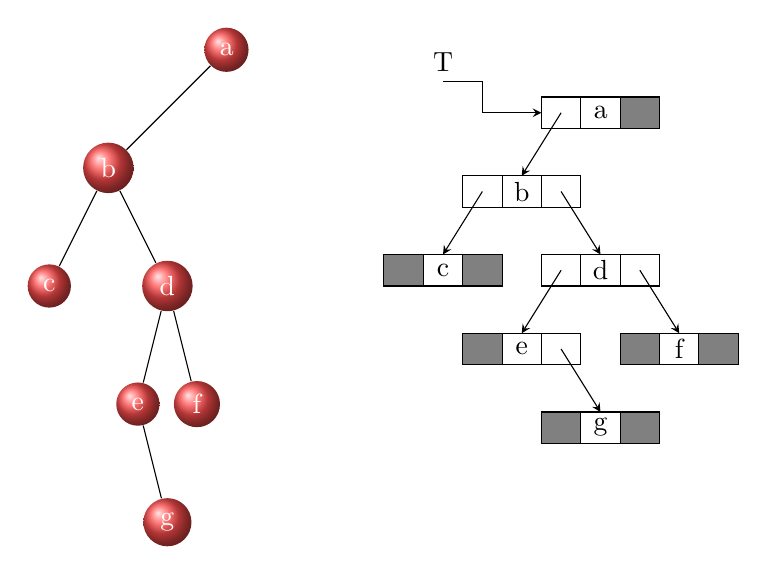
\begin{tikzpicture}
\tikzstyle{every node}=[ball color=red!70,circle,text=white]
\node at (0,0) {a}
child {node {b}
  child {node {c}}
  child {node {d}
    child {node {e}
      child[fill=none] {edge from parent[draw=none]}
      child {node {g}}
    }
    child {node {f}}
  }
}
child[fill=none] {edge from parent[draw=none]};

\tikzstyle{every node}=[]
\def\x{0.5}
\def\y{0.4}

\def\i{8}
\def\j{-1}
\draw[] (\i*\x+0*\x,\j) rectangle (\i*\x+1*\x,\j+\y);
\draw[] (\i*\x+1*\x,\j) rectangle (\i*\x+2*\x,\j+\y);
\filldraw[fill=black!50] (\i*\x+2*\x,\j) rectangle (\i*\x+3*\x,\j+\y);
\node at (\i*\x+1.5*\x,\j+0.5*\y){a};
\draw[->,>=stealth] 
(\i*\x-2.5*\x,\j+1.5*\y)node[above]{T}--(\i*\x-1.5*\x,\j+1.5*\y)--(\i*\x-1.5*\x,\j+0.5*\y)--(\i*\x,\j+0.5*\y);

\def\i{6}
\def\j{-2}
\draw[] (\i*\x+0*\x,\j) rectangle (\i*\x+1*\x,\j+\y);
\draw[] (\i*\x+1*\x,\j) rectangle (\i*\x+2*\x,\j+\y);
\draw[] (\i*\x+2*\x,\j) rectangle (\i*\x+3*\x,\j+\y);
\node at (\i*\x+1.5*\x,\j+0.5*\y){b};

\draw[->,>=stealth] (\i*\x+2.5*\x,\j+1+0.5*\y)--(\i*\x+1.5*\x,\j+\y);

\def\i{4}
\def\j{-3}
\filldraw[fill=black!50] (\i*\x+0*\x,\j) rectangle (\i*\x+1*\x,\j+\y);
\draw[] (\i*\x+1*\x,\j) rectangle (\i*\x+2*\x,\j+\y);
\filldraw[fill=black!50] (\i*\x+2*\x,\j) rectangle (\i*\x+3*\x,\j+\y);
\node at (\i*\x+1.5*\x,\j+0.5*\y){c};

\draw[->,>=stealth] (\i*\x+2.5*\x,\j+1+0.5*\y)--(\i*\x+1.5*\x,\j+\y);


\def\i{8}
\def\j{-3}
\draw[] (\i*\x+0*\x,\j) rectangle (\i*\x+1*\x,\j+\y);
\draw[] (\i*\x+1*\x,\j) rectangle (\i*\x+2*\x,\j+\y);
\draw[] (\i*\x+2*\x,\j) rectangle (\i*\x+3*\x,\j+\y);
\node at (\i*\x+1.5*\x,\j+0.5*\y){d};
\draw[->,>=stealth] (\i*\x+0.5*\x,\j+1+0.5*\y)--(\i*\x+1.5*\x,\j+\y);


\def\i{6}
\def\j{-4}
\filldraw[fill=black!50] (\i*\x+0*\x,\j) rectangle (\i*\x+1*\x,\j+\y);
\draw[] (\i*\x+1*\x,\j) rectangle (\i*\x+2*\x,\j+\y);
\draw[] (\i*\x+2*\x,\j) rectangle (\i*\x+3*\x,\j+\y);
\node at (\i*\x+1.5*\x,\j+0.5*\y){e};
\draw[->,>=stealth] (\i*\x+2.5*\x,\j+1+0.5*\y)--(\i*\x+1.5*\x,\j+\y);


\def\i{10}
\def\j{-4}
\filldraw[fill=black!50] (\i*\x+0*\x,\j) rectangle (\i*\x+1*\x,\j+\y);
\draw[] (\i*\x+1*\x,\j) rectangle (\i*\x+2*\x,\j+\y);
\filldraw[fill=black!50] (\i*\x+2*\x,\j) rectangle (\i*\x+3*\x,\j+\y);
\node at (\i*\x+1.5*\x,\j+0.5*\y){f};
\draw[->,>=stealth] (\i*\x+0.5*\x,\j+1+0.5*\y)--(\i*\x+1.5*\x,\j+\y);


\def\i{8}
\def\j{-5}
\filldraw[fill=black!50] (\i*\x+0*\x,\j) rectangle (\i*\x+1*\x,\j+\y);
\draw[] (\i*\x+1*\x,\j) rectangle (\i*\x+2*\x,\j+\y);
\filldraw[fill=black!50] (\i*\x+2*\x,\j) rectangle (\i*\x+3*\x,\j+\y);
\node at (\i*\x+1.5*\x,\j+0.5*\y){g};

\draw[->,>=stealth] (\i*\x+0.5*\x,\j+1+0.5*\y)--(\i*\x+1.5*\x,\j+\y);
\end{tikzpicture}
\caption{二叉树及其二叉链表}
\end{figure}

\end{frame}
%
\begin{frame}[fragile]\ft{二叉树的链式存储形式}
\begin{figure}
\centering
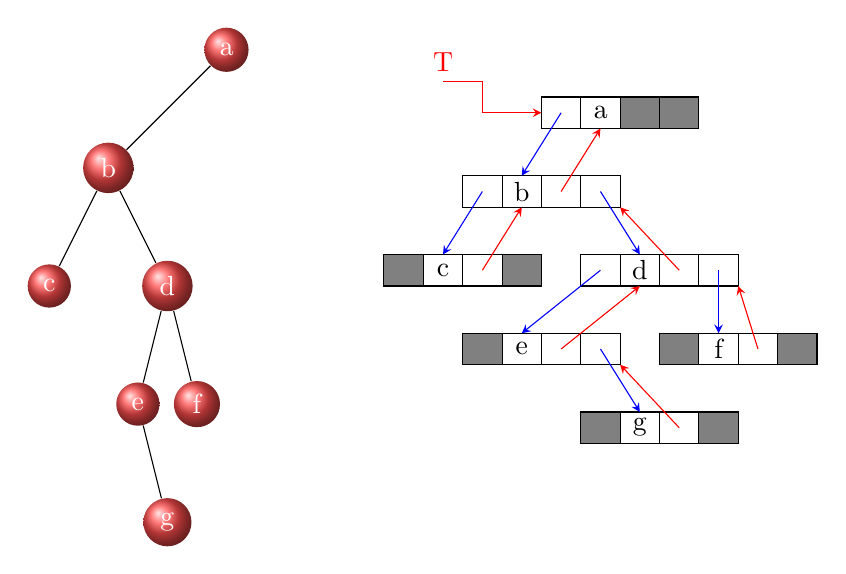
\begin{tikzpicture}
\tikzstyle{every node}=[ball color=red!70,circle,text=white]
\node at (0,0) {a}
child {node {b}
  child {node {c}}
  child {node {d}
    child {node {e}
      child[fill=none] {edge from parent[draw=none]}
      child {node {g}}
    }
    child {node {f}}
  }
}
child[fill=none] {edge from parent[draw=none]};

\tikzstyle{every node}=[]
\def\x{0.5}
\def\y{0.4}

\def\i{8}
\def\j{-1}
\draw[] (\i*\x+0*\x,\j) rectangle (\i*\x+1*\x,\j+\y);
\draw[] (\i*\x+1*\x,\j) rectangle (\i*\x+2*\x,\j+\y);
\filldraw[fill=black!50] (\i*\x+2*\x,\j) rectangle (\i*\x+3*\x,\j+\y);
\filldraw[fill=black!50] (\i*\x+3*\x,\j) rectangle (\i*\x+4*\x,\j+\y);
\node at (\i*\x+1.5*\x,\j+0.5*\y){a};

\draw[red,->,>=stealth] 
(\i*\x-2.5*\x,\j+1.5*\y)node[above]{T}--(\i*\x-1.5*\x,\j+1.5*\y)--(\i*\x-1.5*\x,\j+0.5*\y)--(\i*\x,\j+0.5*\y);

\def\i{6}
\def\j{-2}
\draw[] (\i*\x+0*\x,\j) rectangle (\i*\x+1*\x,\j+\y);
\draw[] (\i*\x+1*\x,\j) rectangle (\i*\x+2*\x,\j+\y);
\draw[] (\i*\x+2*\x,\j) rectangle (\i*\x+3*\x,\j+\y);
\draw[] (\i*\x+3*\x,\j) rectangle (\i*\x+4*\x,\j+\y);
\node at (\i*\x+1.5*\x,\j+0.5*\y){b};

\draw[blue,->,>=stealth] (\i*\x+2.5*\x,\j+1+0.5*\y)--(\i*\x+1.5*\x,\j+\y);
\draw[red,<-,>=stealth] (\i*\x+3.5*\x,\j+1+0.*\y)--(\i*\x+2.5*\x,\j+0.5*\y);

\def\i{4}
\def\j{-3}
\filldraw[fill=black!50] (\i*\x+0*\x,\j) rectangle (\i*\x+1*\x,\j+\y);
\draw[] (\i*\x+1*\x,\j) rectangle (\i*\x+2*\x,\j+\y);
\draw[] (\i*\x+2*\x,\j) rectangle (\i*\x+3*\x,\j+\y);
\filldraw[fill=black!50] (\i*\x+3*\x,\j) rectangle (\i*\x+4*\x,\j+\y);
\node at (\i*\x+1.5*\x,\j+0.5*\y){c};

\draw[blue,->,>=stealth] (\i*\x+2.5*\x,\j+1+0.5*\y)--(\i*\x+1.5*\x,\j+\y);
\draw[red,<-,>=stealth] (\i*\x+3.5*\x,\j+1+0.0*\y)--(\i*\x+2.5*\x,\j+0.5*\y);

\def\i{9}
\def\j{-3}
\draw[] (\i*\x+0*\x,\j) rectangle (\i*\x+1*\x,\j+\y);
\draw[] (\i*\x+1*\x,\j) rectangle (\i*\x+2*\x,\j+\y);
\draw[] (\i*\x+2*\x,\j) rectangle (\i*\x+3*\x,\j+\y);
\draw[] (\i*\x+3*\x,\j) rectangle (\i*\x+4*\x,\j+\y);
\node at (\i*\x+1.5*\x,\j+0.5*\y){d};

\draw[blue,->,>=stealth] (\i*\x+0.5*\x,\j+1+0.5*\y)--(\i*\x+1.5*\x,\j+\y);
\draw[red,<-,>=stealth] (\i*\x+\x,\j+1+0.*\y)--(\i*\x+2.5*\x,\j+0.5*\y);


\def\i{6}
\def\j{-4}
\filldraw[fill=black!50] (\i*\x+0*\x,\j) rectangle (\i*\x+1*\x,\j+\y);
\draw[] (\i*\x+1*\x,\j) rectangle (\i*\x+2*\x,\j+\y);
\draw[] (\i*\x+2*\x,\j) rectangle (\i*\x+3*\x,\j+\y);
\draw[] (\i*\x+3*\x,\j) rectangle (\i*\x+4*\x,\j+\y);
\node at (\i*\x+1.5*\x,\j+0.5*\y){e};

\draw[blue,->,>=stealth] (\i*\x+3.5*\x,\j+1+0.5*\y)--(\i*\x+1.5*\x,\j+\y);
\draw[red,<-,>=stealth] (\i*\x+4.5*\x,\j+1+0.*\y)--(\i*\x+2.5*\x,\j+0.5*\y);

\def\i{11}
\def\j{-4}
\filldraw[fill=black!50] (\i*\x+0*\x,\j) rectangle (\i*\x+1*\x,\j+\y);
\draw[] (\i*\x+1*\x,\j) rectangle (\i*\x+2*\x,\j+\y);
\draw[]  (\i*\x+2*\x,\j) rectangle (\i*\x+3*\x,\j+\y);
\filldraw[fill=black!50](\i*\x+3*\x,\j) rectangle (\i*\x+4*\x,\j+\y);
\node at (\i*\x+1.5*\x,\j+0.5*\y){f};
\draw[blue,->,>=stealth] (\i*\x+1.5*\x,\j+1+0.5*\y)--(\i*\x+1.5*\x,\j+\y);
\draw[red,<-,>=stealth] (\i*\x+2*\x,\j+1+0.*\y)--(\i*\x+2.5*\x,\j+0.5*\y);


\def\i{9}
\def\j{-5}
\filldraw[fill=black!50] (\i*\x+0*\x,\j) rectangle (\i*\x+1*\x,\j+\y);
\draw[] (\i*\x+1*\x,\j) rectangle (\i*\x+2*\x,\j+\y);
\draw[] (\i*\x+2*\x,\j) rectangle (\i*\x+3*\x,\j+\y);
\filldraw[fill=black!50] (\i*\x+3*\x,\j) rectangle (\i*\x+4*\x,\j+\y);
\node at (\i*\x+1.5*\x,\j+0.5*\y){g};

\draw[blue,->,>=stealth] (\i*\x+0.5*\x,\j+1+0.5*\y)--(\i*\x+1.5*\x,\j+\y);
\draw[red,<-,>=stealth] (\i*\x+1*\x,\j+1+0.*\y)--(\i*\x+2.5*\x,\j+0.5*\y);
\end{tikzpicture}
\caption{二叉树及其三叉链表}
\end{figure}

\end{frame}
